\documentclass[a4paper, 12pt, brazilian]{article}

\usepackage{import}
\usepackage{config}

\begin{document}
	\import{sections/}{titlepage}
	
	\tableofcontents
	
	\newpage
	
	\section{Início}
	
	\section{Volume da trincheira}
	
	\begin{equation}
		V_{\textrm{trincheira}}=A_{\textrm{trincheira}}\cdot L=\dfrac{(10+5)\cdot 2}{2}\cdot 600=\SI{9000}{\meter^{3}}
	\end{equation}
	
	\section{Cálculo dos volumes de aterro}
	
	\subsection{Áreas}
	
	\begin{figure}[H]
		\centering
		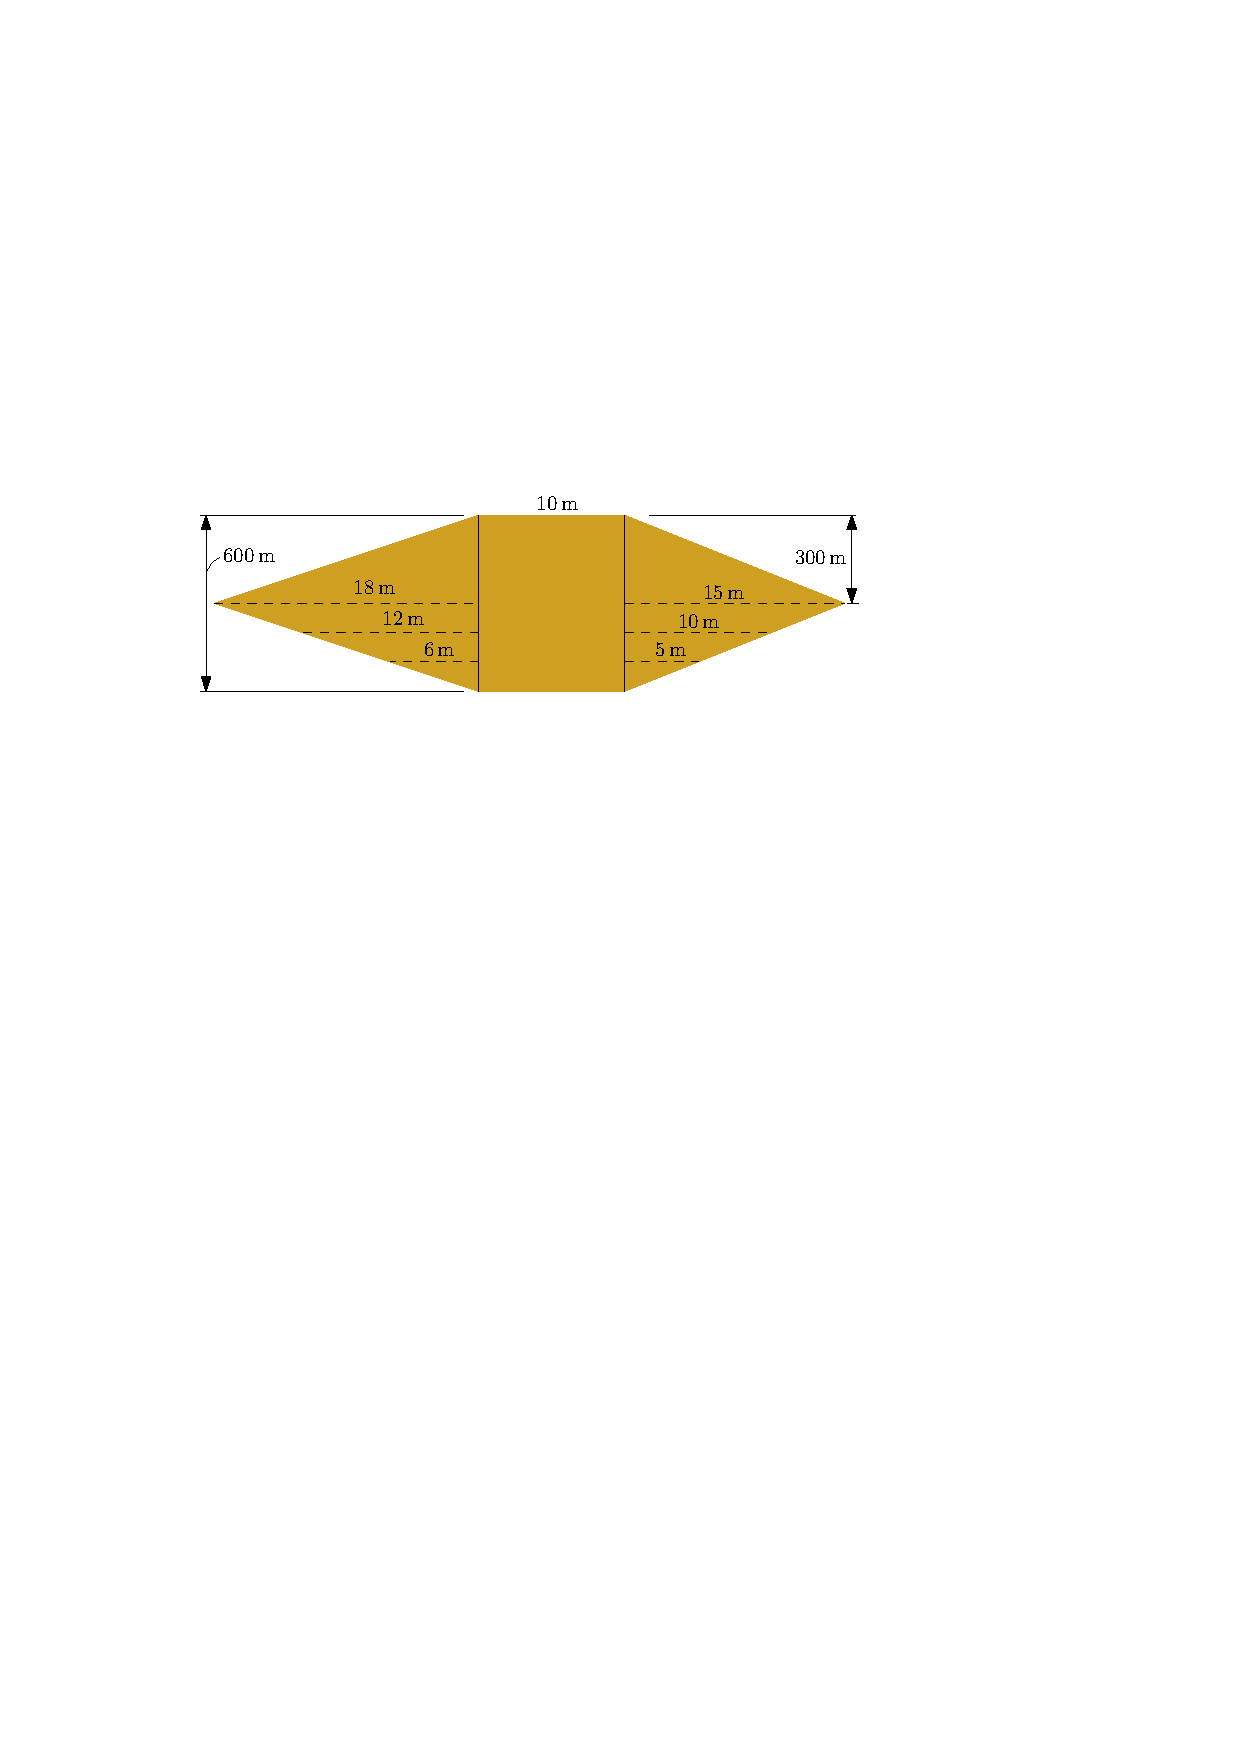
\includegraphics[width=0.9\linewidth]{images/planta}
		\caption{Vista em Planta}
		\label{fig:planta}
	\end{figure}
	
	\begin{small}
		\textit{A partir das proporções estabelecidas para o comprimento L da barragem, foi realizado o cálculo das cotas apresentadas em tracejado para o estudo das seções transversais abaixo, sendo que a seção de maior base tem altura H correspondente a \SI{8}{\meter}}
	\end{small}
	
	\subsubsection{Seção central}
	\begin{figure}[H]
		\centering
		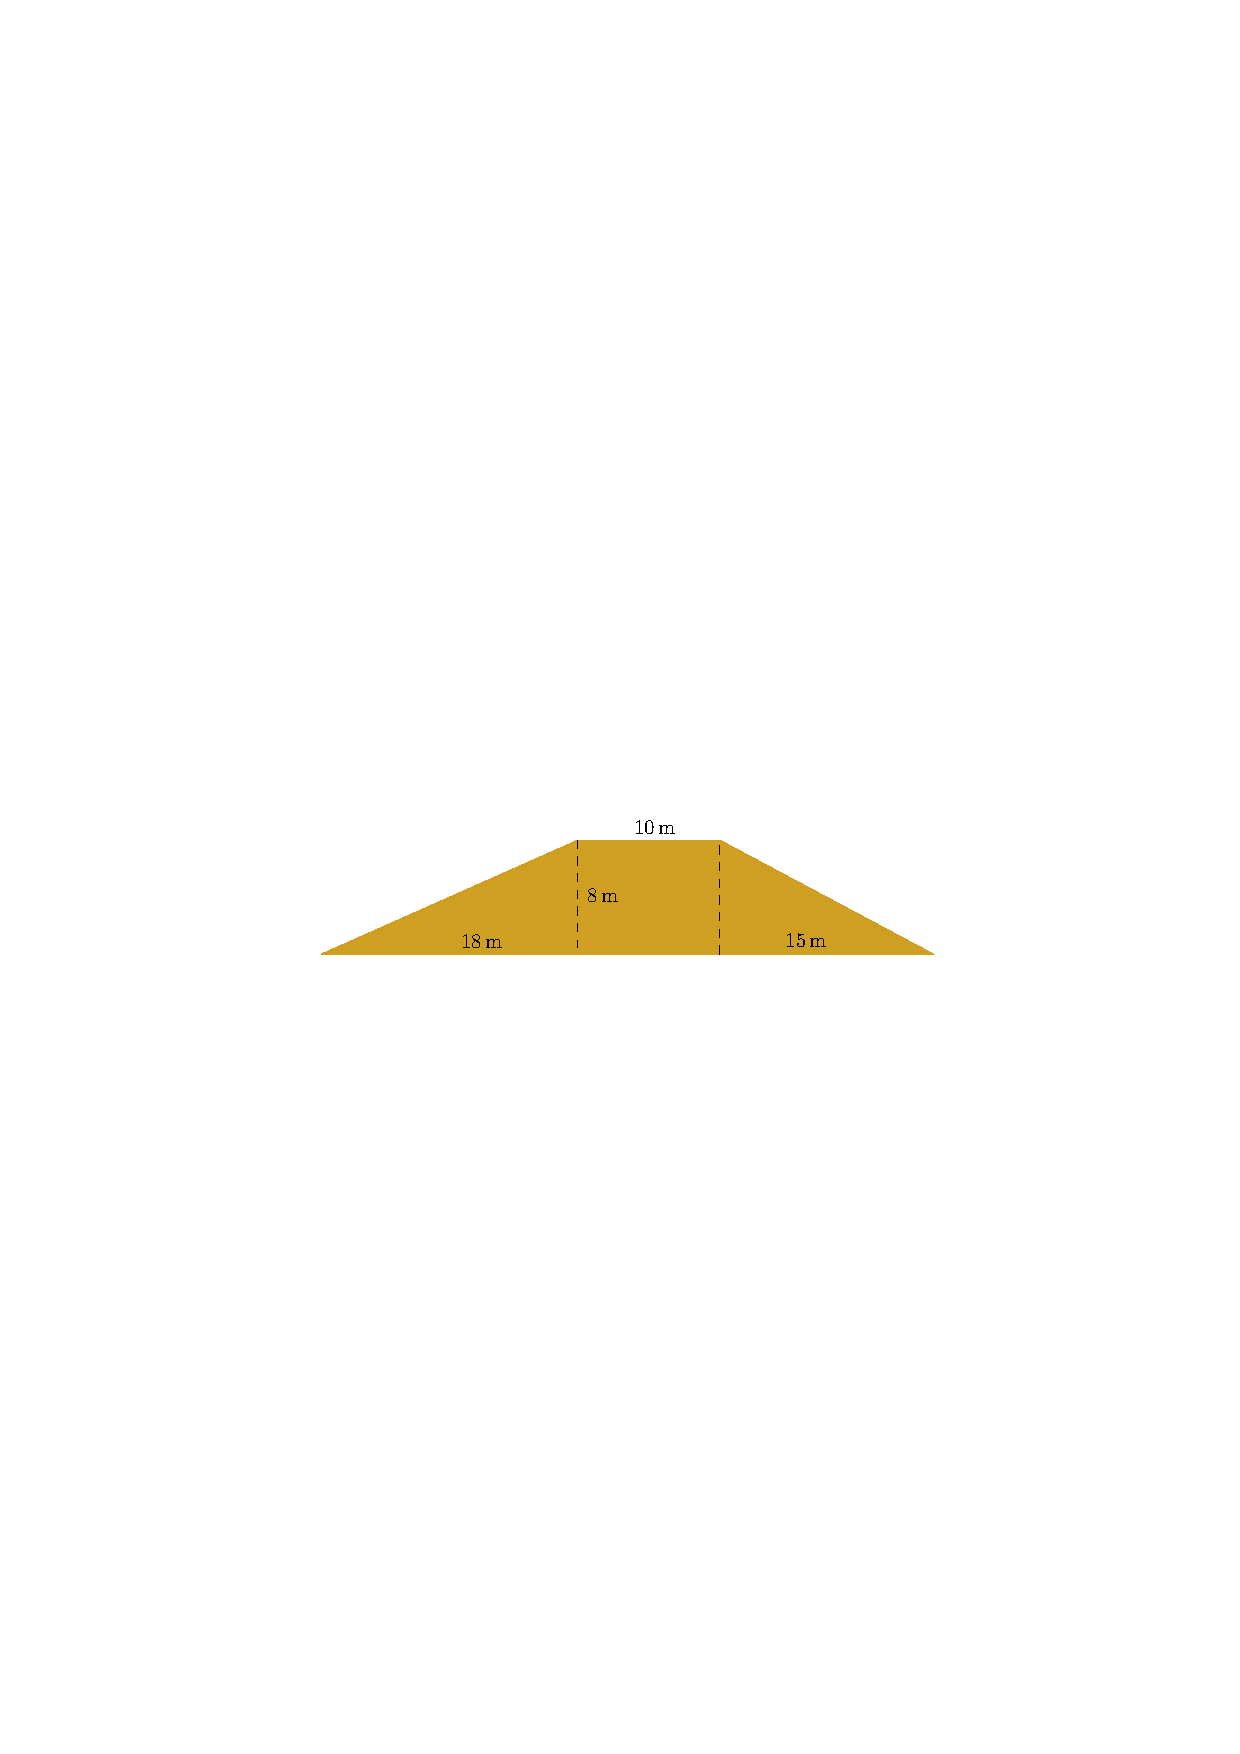
\includegraphics[width=0.85\linewidth]{images/center}
		\label{fig:center}
	\end{figure}
	
	
	\begin{eqnarray}
		A_{1}&=&\dfrac{(B+b)\cdot h}{2}\\
		&=&\dfrac{(18+15+10+10)\cdot 8}{2}
		=\SI{212}{\meter^{2}}
	\end{eqnarray}
	
	
	\subsubsection{Seção transversal em $L/6=\SI{100}{\meter}$}
	\begin{figure}[H]
		\centering
		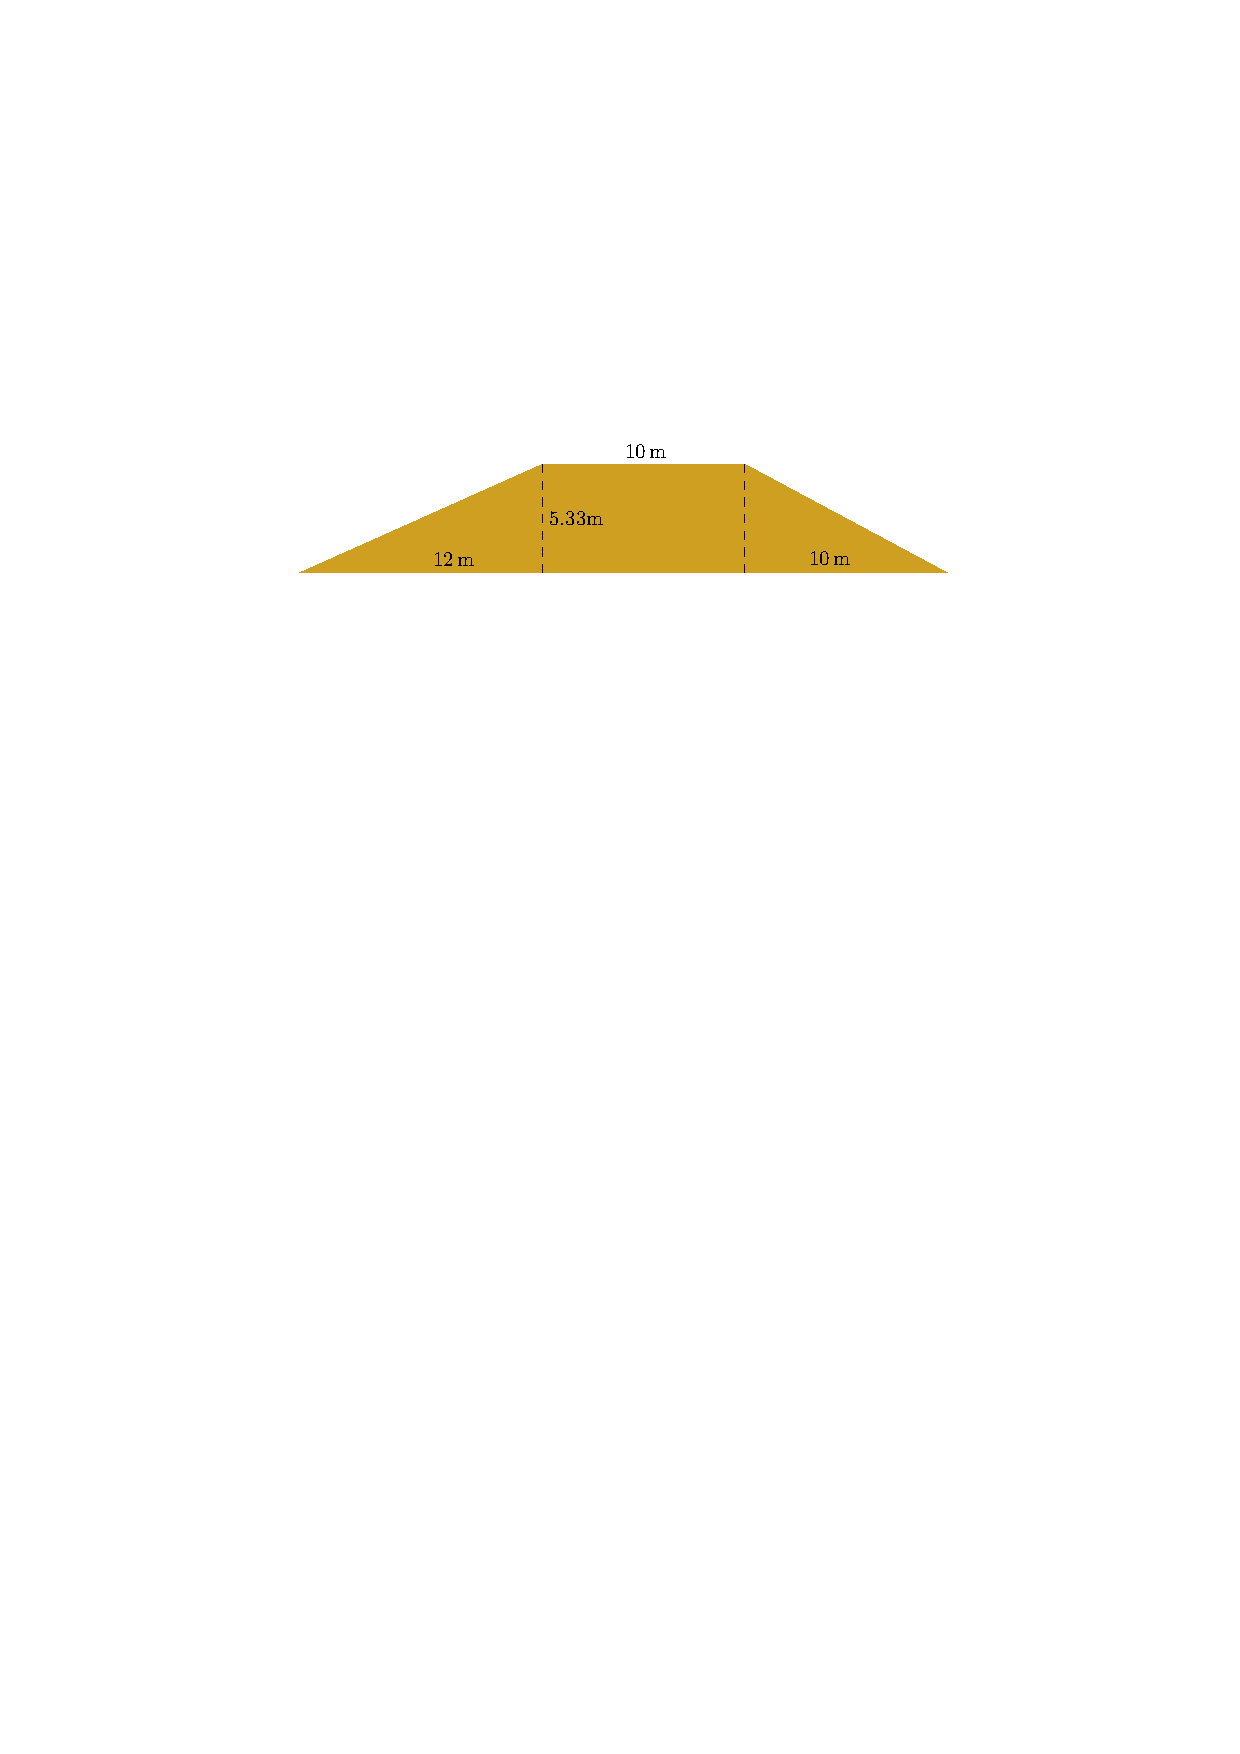
\includegraphics[width=0.9\linewidth]{images/lpersix}
		\label{fig:lpersix}
	\end{figure}
	
	
	\begin{eqnarray}
		A_{2}&=&\dfrac{(12+10+10+10)\cdot 5.333}{2}\\
		&=&\SI{111.73}{\meter^{2}}
	\end{eqnarray}
	
	\subsubsection{Seção transversal em $2L/6=\SI{200}{\meter}$}
	\begin{figure}[H]
		\centering
		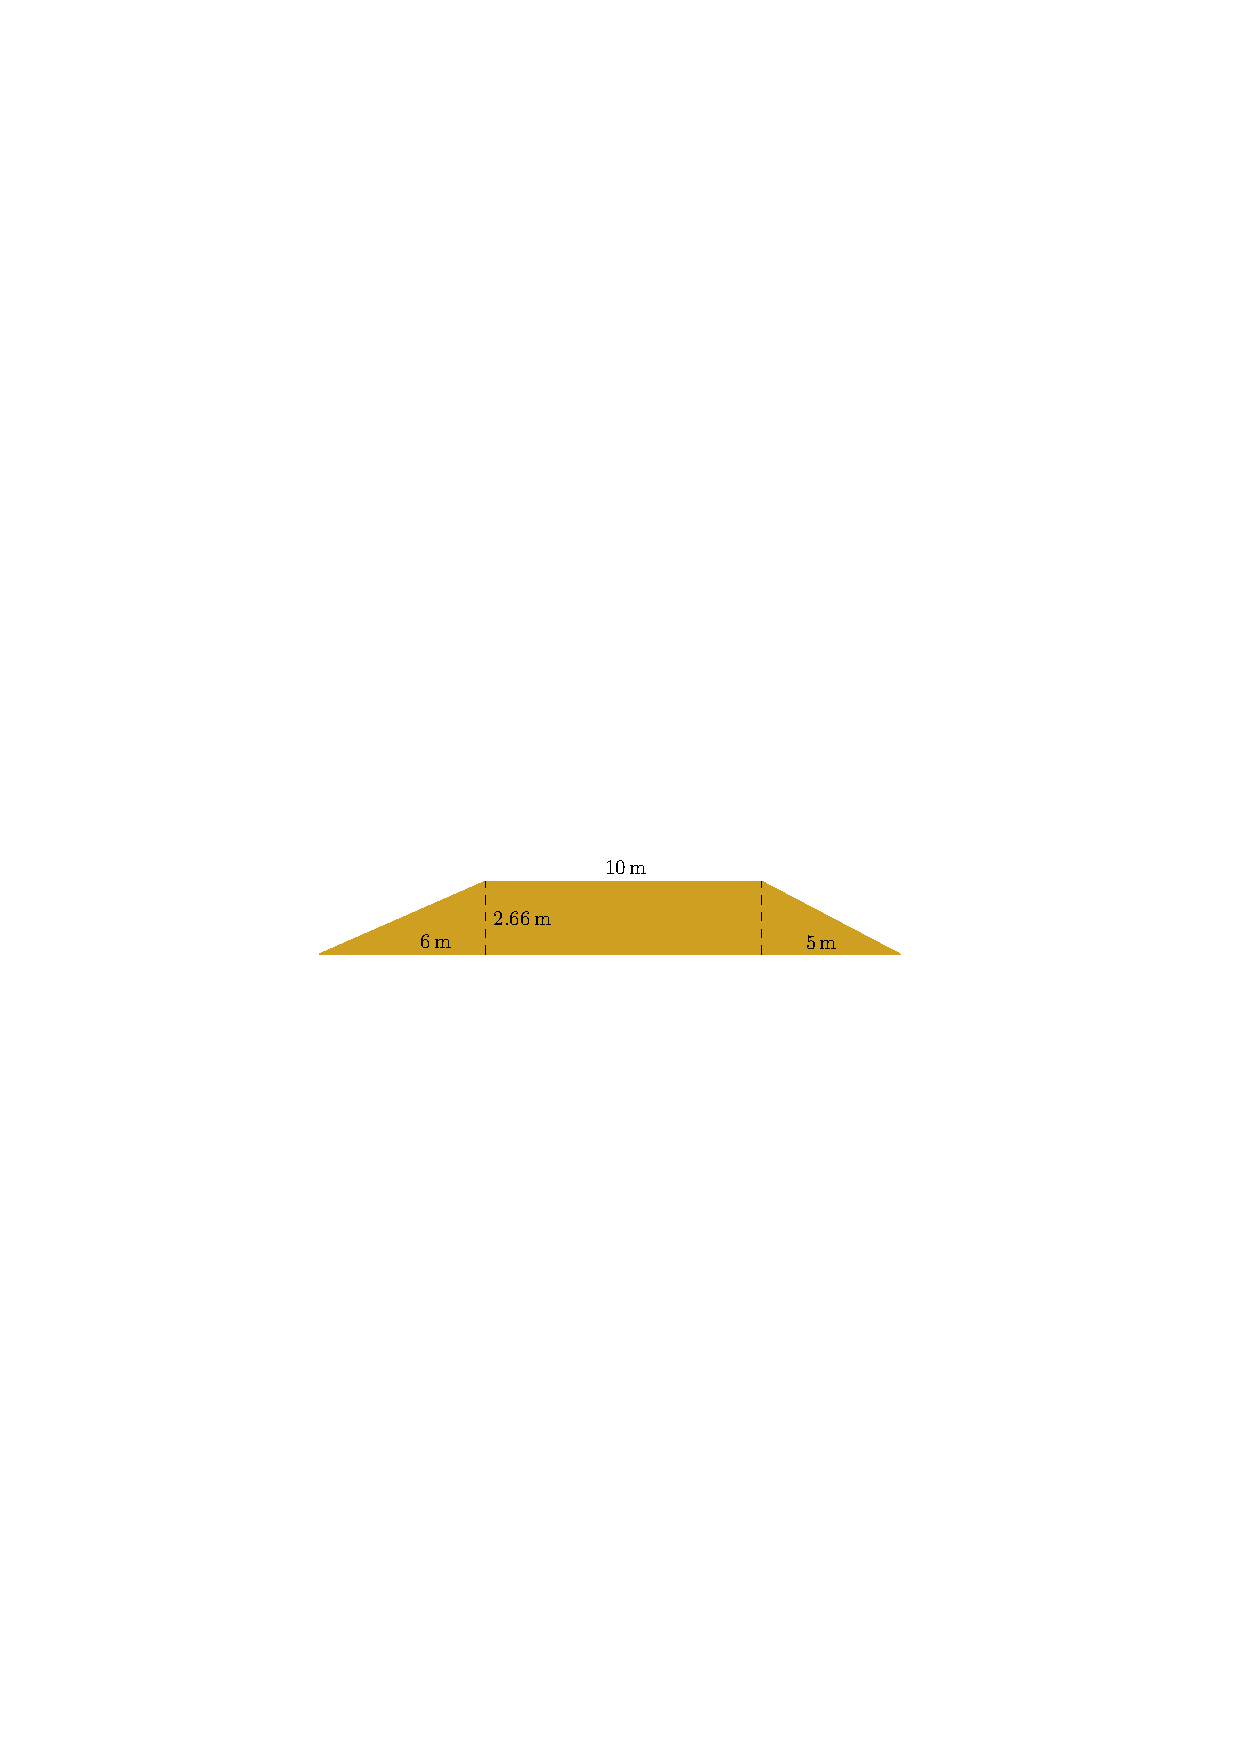
\includegraphics[width=0.85\linewidth]{images/twolpersix}
		\label{fig:twolpersix}
	\end{figure}
	
	\begin{eqnarray}
		A_{3}&=&\dfrac{(10+10+6+5)\cdot 2.666}{2}\\
		&=&\SI{41.33}{\meter^{2}}
	\end{eqnarray}
	
	\subsection{Volumes}
	\begin{eqnarray}
		V_{1}&=&\left(\dfrac{A_{1}+A_{2}}{2}\right)\cdot\dfrac{L}{6}=\SI{16196.5}{\meter^{3}}
	\end{eqnarray}
	
	\begin{eqnarray}
		V_{2}&=&\left(\dfrac{A_{2}+A_{3}}{2}\right)\cdot\dfrac{L}{6}=\SI{7663}{\meter^{3}}	
	\end{eqnarray}
	
	\begin{eqnarray}
		V_{1}&=&\left(\dfrac{A_{2}+A_{3}}{2}\right)\cdot\dfrac{L}{6}=\SI{2066.5}{\meter^{3}}
	\end{eqnarray}
	
	Somando as três porções de volume, obtemos metade do total
	
	\begin{equation}
		V_{T}'=\sum\limits_{i=1}^{3}V_{i}=\SI{25926}{\meter^{3}}
	\end{equation}
	
	portanto o volume de aterro total será 
	
	\begin{equation}
		V_{T}=2V_{T}'=\SI{51852}{\meter^{3}}
	\end{equation}
	
	\section{Volume do \textit{rip-rap}}
	\begin{eqnarray}
		V_{\textit{rip-rap}}&=&\sqrt{H^{2}+V^{2}}\cdot L\cdot\textrm{espessura}\\
		&=&\sqrt{2.5^{2}+7.5^{2}}\cdot 600\cdot 0.3\\
		\therefore V_{\textit{rip-rap}}&=&\SI{1423.025}{\meter^{3}}
	\end{eqnarray}
	
	\section{Área de grama}
	\begin{eqnarray}
		A_{\textrm{grama}}&=&\dfrac{\sqrt{8^{2}+15^{2}}\cdot 600}{2}\\
		&=&\SI{5100}{\meter^{2}}
	\end{eqnarray}
	
	\section{Filtro horizontal}
	\begin{eqnarray}
		V_{FH}&=&\dfrac{l\,L\,\textrm{espessura}}{2}\\
		&=&\dfrac{15\cdot 600\cdot 0.7}{2}\\
		&=&\SI{3150}{\meter^{3}}
	\end{eqnarray}
	
	\section{Filtro vertical}
	\begin{eqnarray}
		V_{FV}&=&\dfrac{8\cdot 600\cdot 0.5}{2}\\
		&=&\SI{1200}{\meter^{3}}
	\end{eqnarray}
	
	\section{Seção do sangradouro}
	
	Para o cálculo, considerou-se $H=0.5$ (mínimo permitido para pequenas barragens), assim
	\begin{eqnarray}
		Q&=&1.55\,L\,H^{1.5}\\
		1&=&1.55\cdot L\cdot 0.5^{1.5}\\
		L&=&\SI{1.82}{\meter}
	\end{eqnarray}
	
	\begin{figure}[H]
		\centering
		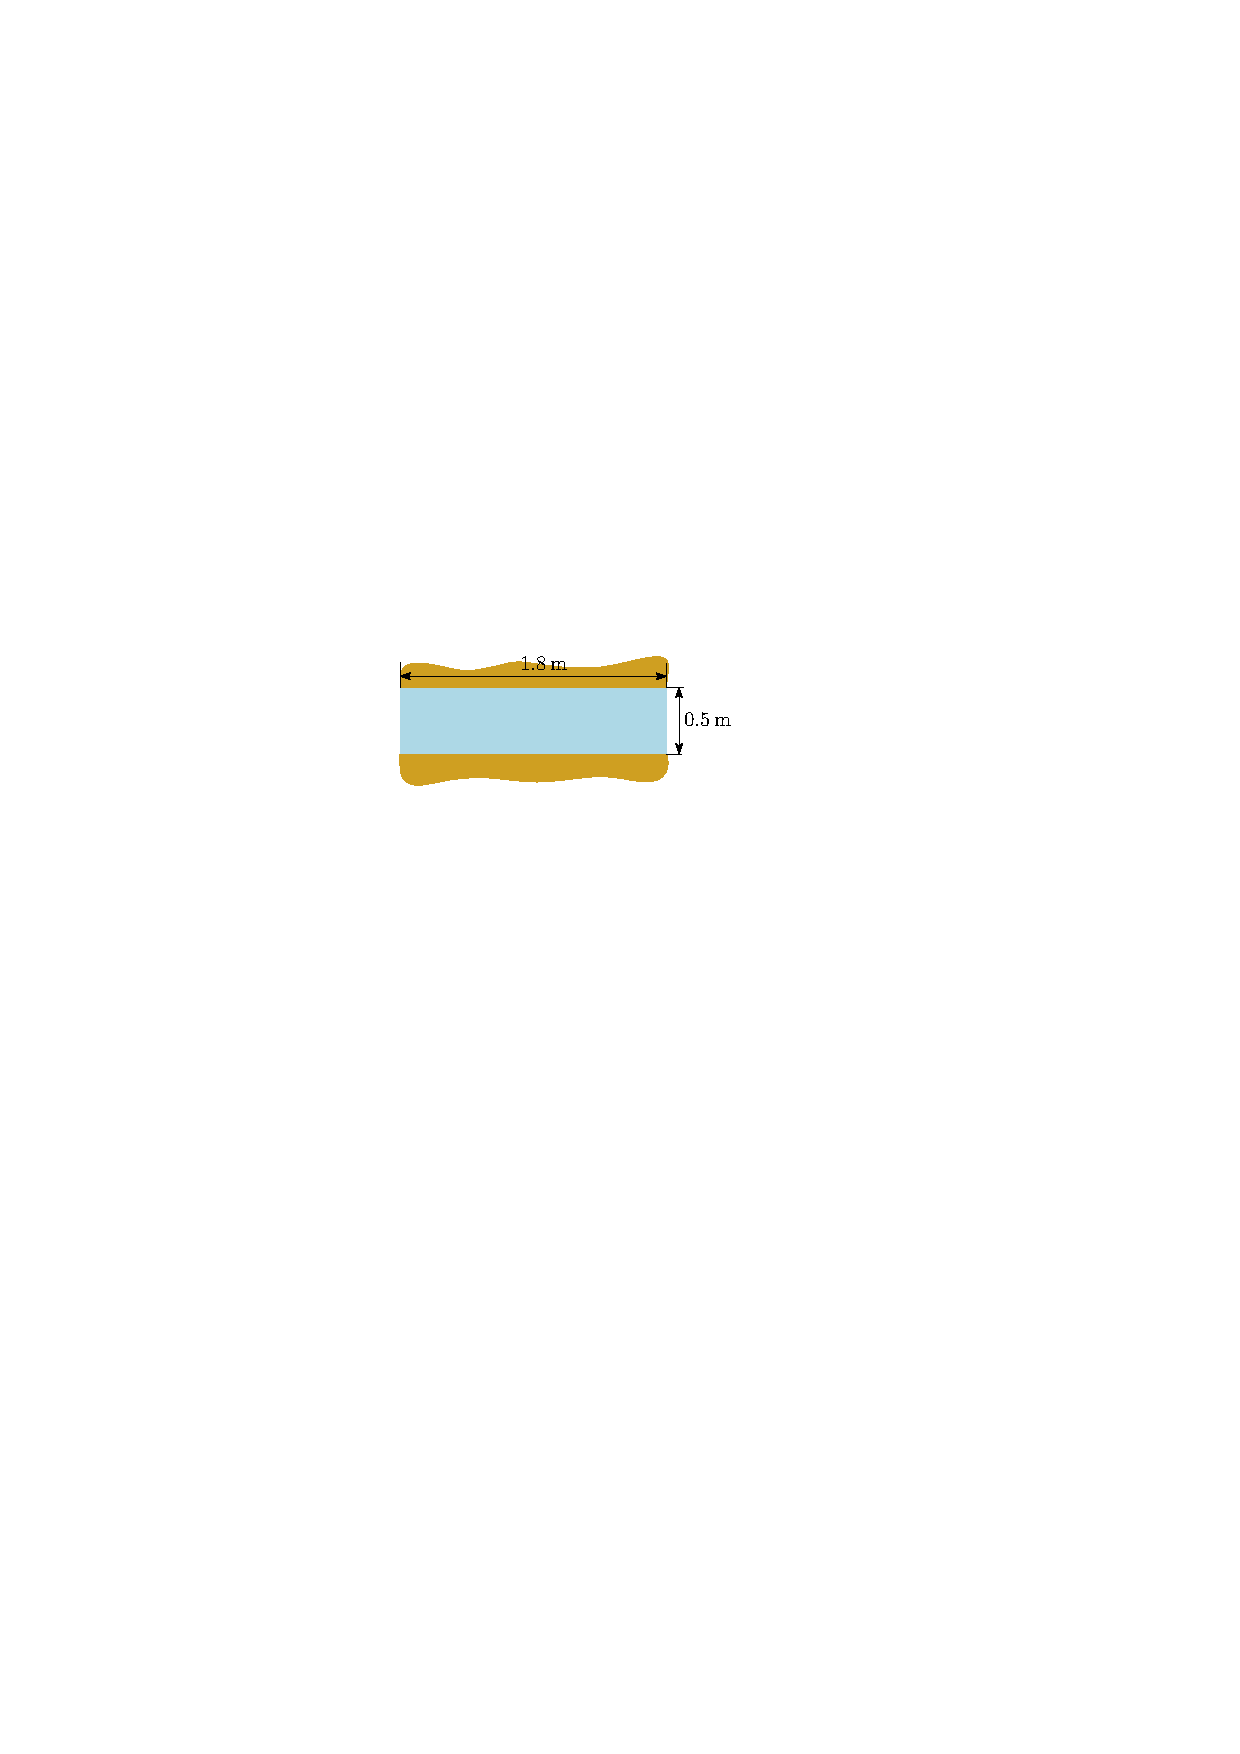
\includegraphics[width=0.5\linewidth]{images/sang}
		\label{fig:sang}
	\end{figure}
	
	\newpage
	\section{Tabela de custos}
	
	\import{sections}{data}
	
	\begin{small}
		\begin{itemize}
			\item\textit{O anteprojeto para uma barragem de $\SI{20000}{\meter^{3}}$ é de \textrm{R\$15\,000,00}, portanto, para o volume de aterro de $\SI{51852}{\meter^{3}}$ foi sugerido o dobro do custo da anterior.}
			\item\textit{Foi proposto um custo adicional de R\$1000,00, tendo em vista a análise inicial requerida no local, exigindo transporte e custos com a agrimensura.}
		\end{itemize}
	\end{small}
	
	\newpage
	
	\section{Orçamento de terraplenagem}
	
	\subsection{Equipamentos para terraplenagem}
	
	\import{sections/}{terra}
	
	\subsubsection{Custo estimado}
	
	\noindent 03 escavadeiras hidráulicas sobre esteiras: $\SI{1230}{\hour}\times\textrm{R\$}300,00$
	
	\noindent 09 a 12 caminhões traçados ($\SI{12}{\meter^{3}}$): $\SI{1080}{\hour}\times\textrm{R\$}140,00$
	
	\noindent 03 tratores de lâmina sobre esteiras (CAT D6): $\SI{1080}{\hour}\times\textrm{R\$}250,00$
	
	\noindent 03 rolos compactadores (CA25 ou similar):  $\SI{1080}{\hour}\times\textrm{R\$}180,00$
	
	\noindent 03 tratores agrícolas com grade: $\SI{1080}{\hour}\times\textrm{R\$}130,00$
	
	\noindent 03 caminhões irrigadeira:  $\SI{600}{\hour}\times\textrm{R\$}140,00$
	
	\# Valor total estimado dos equipamentos: \textbf{R\$1\,209\,000,00}
	\vspace{1cm}

	\small{\textit{Obs: Os valores foram extraídos do roteiro presente no Moodle. Ao levar em conta que a barragem dimensionada nessa situação equivale a quase três vezes a do roteiro \textrm{($\SI{20000}{\meter^{3}}$)}, ao considerar o mesmo ritmo de horas requeridas para o cumprimento da operação, os equipamentos foram redimensionados de forma proporcional.}}
	
\end{document}